\section[REVISÃO DA LITERATURA]{revisão da literatura}

A pesquisa da base bibliográfica utilizada neste trabalho considerou a busca por livros,
teses, monografias e artigos nas seguintes fontes especializadas: PubMed, ACM
(Association for Computing Machinery), IEEE (Institute of Electrical and Electronics
Engineers), RadiologySource, Radiographics, USP (Universidade de São Paulo), UFSC
(Universidade Federal de Santa Catarina) e IBICT (Instituto Brasileiro de Informações em
Ciência e Tecnologia).

O PubMed é uma base de dados que permite a pesquisa bibliográfica de artigos
publicados em revistas de grande circulação da área médica. Ele foi desenvolvido pelo
NCBI (National Center for Biotechnology Information), sendo mantido pela NLM
(National Library of Medicine). ...

...
A Figura \ref{esquematico} mostra, respectivamente, um diagrama esquemático de um equipamento de
mamografia e um desenho ilustrativo de um mamógrafo.

\begin{figure}[ht]
 \centering
 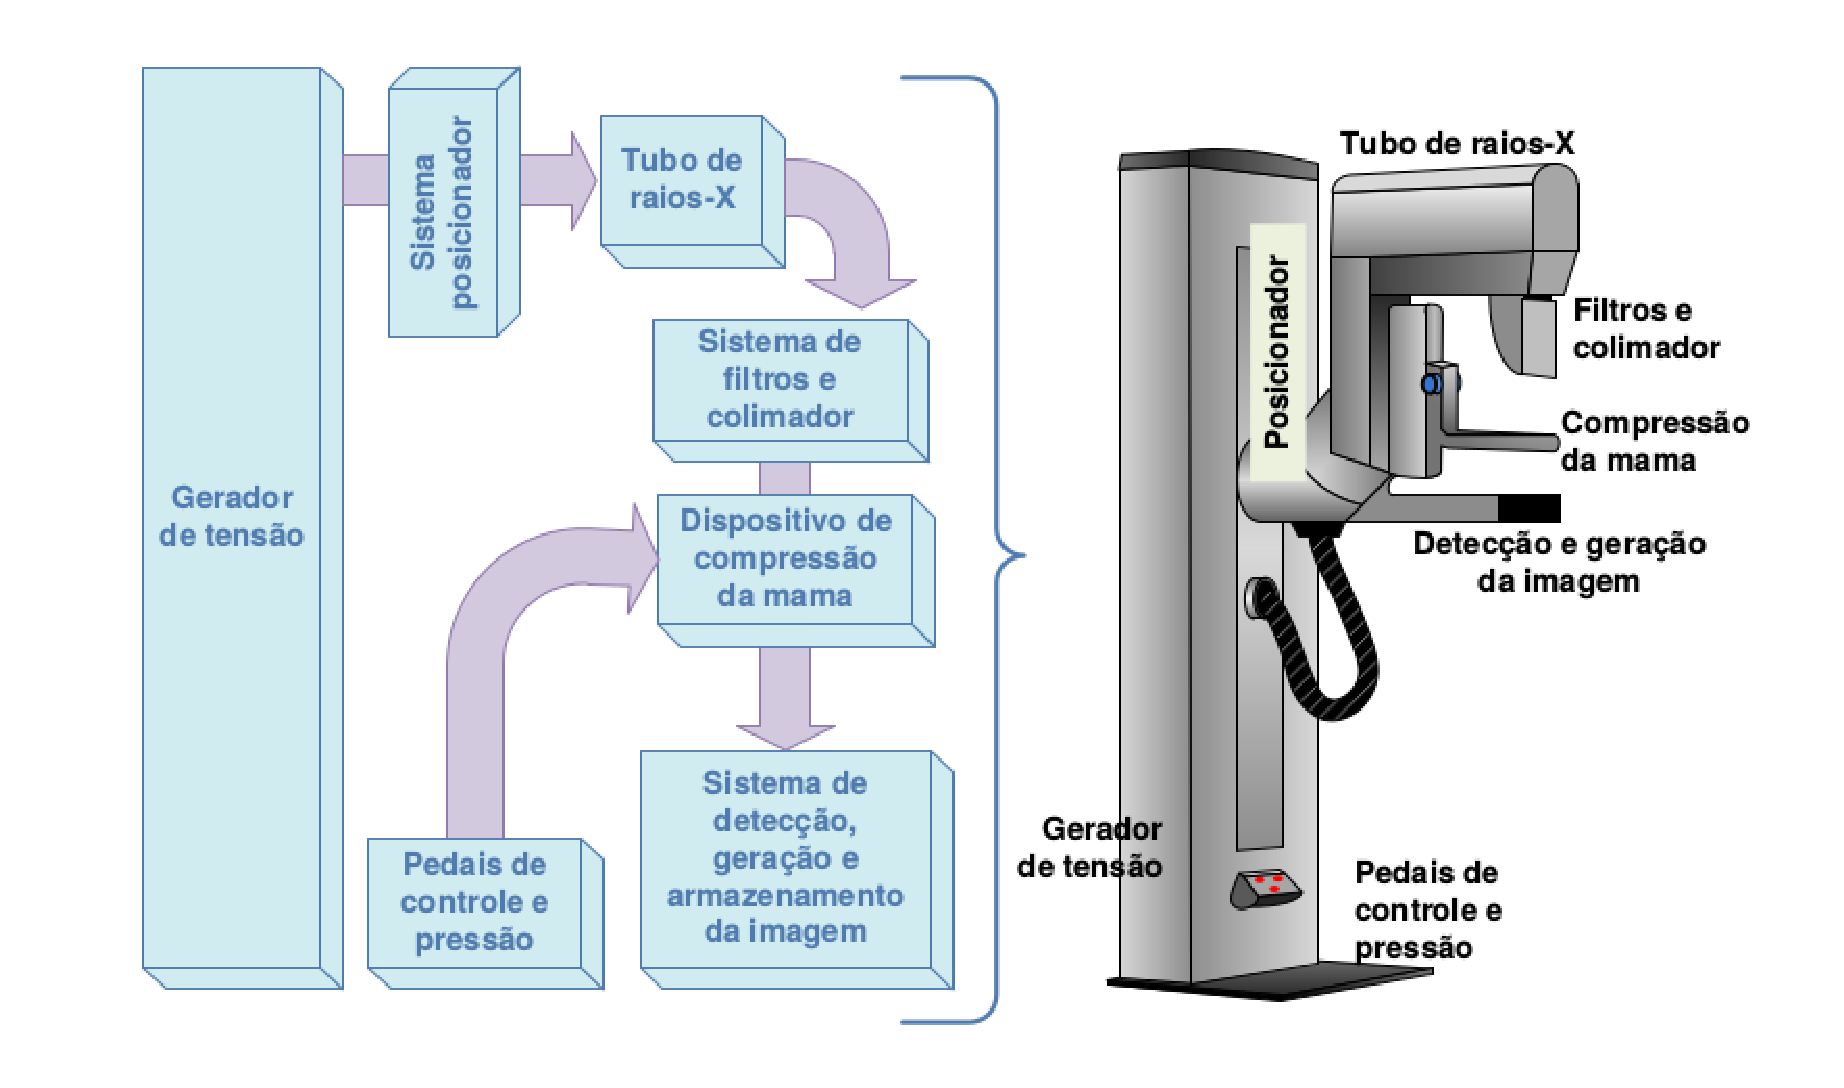
\includegraphics[scale=0.45]{figuras/fig1.eps}
 \caption{Esquemático do mamógrafo (Modificado de MINISTÉRIO DA SAÚDE, 2002).}
 \label{esquematico}
\end{figure}





